\PassOptionsToPackage{unicode,pdfusetitle}{hyperref}
\PassOptionsToPackage{hyphens}{url}
\PassOptionsToPackage{dvipsnames,svgnames,x11names}{xcolor}

\documentclass[english,a4paper]{article}
\usepackage[margin=1in]{geometry}

\usepackage{lmodern}
\usepackage{amssymb,amsmath,amsthm,mathtools,isomath}

\usepackage[T1]{fontenc}
\usepackage[utf8]{inputenc}
\usepackage{textcomp} % provide euro and other symbols
\usepackage{babel}

\usepackage{upquote} % straight quotes in verbatim environments
\usepackage{nicefrac}	% compact symbols for 1/2, etc.
\usepackage[]{microtype}
\UseMicrotypeSet[protrusion]{basicmath} % disable protrusion for tt fonts

\usepackage{xcolor}
\usepackage{xurl}
\usepackage{bookmark}
\usepackage{csquotes}
\usepackage{siunitx}
\usepackage{enumitem}


\usepackage{algorithm,algpseudocode}
\usepackage[titlenumbered,linesnumbered,ruled,noend,algo2e]{algorithm2e}

\usepackage[textsize=scriptsize]{todonotes}
\newcommand{\mathurin}[1]{\textcolor{purple}{[MM: #1]}}
\newcommand{\johan}[1]{\textcolor{RoyalBlue}{[JL: #1]}}
\newcommand{\jonas}[1]{\textcolor{red!20}{[JW: #1]}}
\newcommand{\jw}[1]{\todo[color=red!20]{{\bf JW:} #1}}
\newcommand{\mm}[1]{\todo[color=purple!20]{{\bf Mathurin:} #1}}
\newcommand{\klopfe}[1]{\todo[color=orange]{{\bf Klopfe:} #1}}
\newcommand{\qk}[1]{\textcolor{orange}{#1}}
\newcommand{\jl}[1]{\todo[color=black!30]{{\bf JL:} #1}}
\newcommand{\JL}[1]{{\todo[inline,color=black!30]{{\bf JL:} #1}}}

\newcommand{\widebar}[1]{\mkern 1.5mu\overline{\mkern-1.5mu#1\mkern-1.5mu}\mkern 1.5mu}

\usepackage[noabbrev,nameinlink]{cleveref}

\usepackage{hyperref}
\hypersetup{
  colorlinks = true,
  linkcolor  = RoyalBlue4,
  filecolor  = RoyalBlue4,
  citecolor  = VioletRed4,
  urlcolor   = RoyalBlue4
}

\usepackage{longtable}
\usepackage{booktabs}

\usepackage{etoolbox}

% Allow footnotes in longtable head/foot
\usepackage{footnotehyper}
\makesavenoteenv{longtable}

\usepackage{graphicx}
\graphicspath{{../figures/}}
\usepackage{subcaption}

% % tikz
% \usepackage{pgfplots}
% \pgfplotsset{width=7cm,compat=1.16}
% \usepgfplotslibrary{external}
% \tikzexternalize

% Set default figure placement to htbp
\makeatletter
\def\fps@figure{htbp}
\makeatother

\usepackage{pdfpages}

\usepackage[]{authblk}
\renewcommand\Affilfont{\itshape\small}

% bibliography
\makeatletter
\def\blx@nowarnpolyglossia{}
\makeatother
\usepackage[citestyle=alphabetic,language=english]{biblatex}
\addbibresource{slopecd.bib}

\setlength{\emergencystretch}{3em} % prevent overfull lines

% operators
\DeclareMathOperator*{\argmax}{arg\,max}
\DeclareMathOperator*{\argmin}{arg\,min}
\DeclareMathOperator{\tr}{tr}
\DeclareMathOperator{\diag}{diag}
\DeclareMathOperator{\range}{range}
\DeclareMathOperator{\nullspace}{null}
\DeclareMathOperator{\rank}{rank}
\DeclareMathOperator{\card}{card}
\DeclareMathOperator{\sign}{sign}


\newcommand{\abs}[1]{\lvert {#1} \rvert}
\newcommand{\norm}[1]{\lVert {#1} \rVert}
% theorems
\theoremstyle{plain}
\newtheorem{theorem}{Theorem}[section]
\newtheorem{proposition}[theorem]{Proposition}
\newtheorem{lemma}[theorem]{Lemma}
\newtheorem{corollary}[theorem]{Corollary}
\theoremstyle{definition}
\newtheorem{definition}[theorem]{Definition}
\newtheorem{assumption}[theorem]{Assumption}
\theoremstyle{remark}
\newtheorem{remark}[theorem]{Remark}
\newtheorem{example}{Example}

% mathbb and mathcal letters
\newcommand{\bbR}{\mathbb{R}}
\newcommand{\cB}{\mathcal{B}}
\newcommand{\cC}{\mathcal{C}}

% title block
\title{Coordinate Descent for SLOPE}
\author[1,*]{}
\affil[1]{Department of Statistics, Lund University}
\affil[*]{Corresponding author: \href{}{}}
\date{\today}

\begin{document}

\maketitle

\begin{abstract}
  %!TEX root=./main.tex
The lasso is the most famous sparse regression and feature selection method.
One reason for its popularity is the speed at which the underlying optimization problem can be solved.
Sorted L-One Penalized Estimation (SLOPE) is a generalization of the lasso with appealing statistical properties.
In spite of this, the method has not yet reached widespread interest.
A major reason for this is that current software packages that fit SLOPE rely on algorithms that perform poorly in high dimensions. 
To tackle this issue, we propose a new fast algorithm to solve the SLOPE optimization problem,
which combines proximal gradient descent and proximal coordinate descent steps.
We provide new results on the directional derivative of the SLOPE penalty and its related SLOPE thresholding operator, as well as provide convergence guarantees for our proposed solver.
In extensive benchmarks on simulated and real data, we demonstrate our method's performance against a long list of competing algorithms.

\end{abstract}

%!TEX root = ./main.tex
\section{Introduction}\label{sec:introduction}
%%%%%%%%%%%%%%%%%%%%%%%%%%%%%%%%%%%%%%%%%%%%%%

In this paper we present a novel numerical algorithm for Sorted L-One Penalized
Estimation (SLOPE)~\parencite{bogdan2013,bogdan2015,zeng2014ordered}, defined as
\begin{problem}\label{pb:slope}
  \min_{\beta \in \mathbb{R}^p}
  P(\beta) = F(\beta) + J(\beta)
\end{problem}
% \mm{TODO change}
where we take \(F\) to be smooth and twice differentiable and
% \mm{to discuss: $L(X\beta)$ doable? + some computation are sepcific to  the quadratic case}
\begin{equation}
  \label{eq:sorted-l1-norm}
  J(\beta) = \sum_{j=1}^p \lambda_j|\beta_{(j)}|
\end{equation}
is the \emph{sorted \(\ell_1\) norm}, defined through
\begin{equation*}
  |\beta_{(1)}| \geq |\beta_{(2)}| \geq \cdots \geq |\beta_{(p)}| \enspace,
\end{equation*}
with \(\lambda\) being a fixed non-increasing and non-negative sequence.

The sorted $\ell_1$ norm is a sparsity-enforcing penalty that has become
increasingly popular due to several appealing properties, such as its ability
to control false discovery rate~\parencite{bogdan2015,kos2020}, cluster
coefficients~\parencite{figueiredo2016, schneider2020a}, and recover sparsity and
ordering patterns in the solution~\parencite{bogdan2022}. Unlike other competing
sparse regularization methods such as MCP~\parencite{zhang2010} and
SCAD~\parencite{fan2001}, SLOPE is also a convex problem~\parencite{bogdan2015}.

In spite of the availability of predictor screening
rules~\parencite{larsson2020c,elvira2022}, which help speed up SLOPE in the
high-dimensional regime, current state-of-the-art algorithms for SLOPE perform
poorly in comparison to those of more established penalization methods such as
the lasso (\(\ell_1\)-norm regularization) and ridge regression
(\(\ell_2\)-norm regularization).
As a small illustration of this issue, we compared the speed at which the \pkg{SLOPE}~\parencite{friedman2022} and \pkg{glmnet}~\parencite{friedman2022} packages solve a SLOPE and lasso problem, respectively, for the \dataset{bcTCGA} data set.
In this small experiment, \pkg{SLOPE} takes 42.7 seconds to reach convergence, whilst \pkg{glmnet} requires only 0.143 seconds\footnote{See~\Cref{sec:slope-vs-glmnet} for details on how this experiment was run.}.

This lackluster performance has hampered the applicability of SLOPE to many
real-world applications. A major reason for why algorithms for solving
$\ell_1$-, MCP-, or SCAD-regularized problems enjoy better performance is that
they use coordinate
descent~\parencite{tseng2001convergence,friedman2010,breheny2011}. Current SLOPE
solvers, on the other hand, rely on proximal gradient descent algorithms such
as FISTA~\parencite{beck2009} and the alternating direction method of multipliers
method (ADMM)~\parencite{boyd2010}, which have proven to be less inefficient than
coordinate descent in empirical benchmarks on related problems, such as the
lasso~\parencite{moreau2022benchopt}. Applying coordinate descent to SLOPE is not,
however, straightforward since convergence guarantees for coordinate descent
require the objective to be separable, which is not the case for SLOPE. As a
result, naive coordinate descent schemes can get
stuck~(\Cref{fig:naive-cd-stuck}).

\begin{figure}[htb]
  \centering
  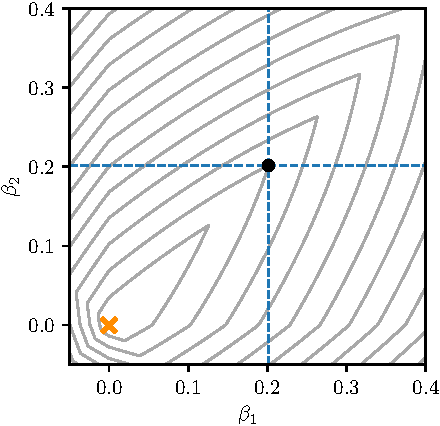
\includegraphics[]{naive-cd-stuck.pdf}
  \caption{%
    An example of (standard) coordinate descent getting stuck on a two-dimensional SLOPE problem.
    The main plot shows level curves for the primal objective~\eqref{pb:slope}, with the optimum \(\beta^* = [0, 0]^T\) indicated by the orange cross.
    The marginal plots displays objective values at \(\beta_1 = 0.2\) when optimizing over \(\beta_2\) and vice versa.
    At \(\beta = [0.2,0.2]^T\), a naive coordinate descent algorithm can only move in the directions indicated by the dashed lines---neither of which are descent directions for the objective.
    As a result, the algorithm is stuck.
  }
  \label{fig:naive-cd-stuck}
\end{figure}

In this article we address this problem by introducing a new, highly effective
algorithm for SLOPE based on a hybrid proximal gradient and coordinate descent
scheme. Our method features convergence guarantees and reduces the time
required to fit SLOPE by orders of magnitude in our empirical experiments.

\subsection{Notation}\label{sec:notation}

Let \((i)^{-}\) be the inverse of \((i)\) such that
\(\big((i)\big)^- = i\).
\begin{example}
  \begin{tabular}{cccc}
    \toprule
    \(i\) & \(\beta\) & \((i)\) & \((i)^-\) \\
    \midrule
    1     & 1         & 2       & 3         \\
    2     & -3        & 3       & 1         \\
    3     & 2         & 1       & 2         \\
    \bottomrule
  \end{tabular}
\end{example}
Note that this means that
\[
  J(\beta) = \sum_{j=1}^p \lambda_j |\beta_{(j)}|
           = \sum_{j=1}^p \lambda_{(j)^-}|\beta_j|.
\]

Furthermore, let
\[
  S(\mathcal{A}) = \sum_{i \in \mathcal{A}} \lambda_{(i)^-}.
\]

Also, let \(\mathcal{C}_1, \mathcal{C}_2\, \dots, \mathcal{C}_m\) be the
clusters such that
\[
  \mathcal{C}_i = \{j : |\beta_j| = c_i\} \quad \text{and} \quad
  c_1 > c_2 > \cdots \geq 0.
\]
In addition, let \(C(\alpha)\) be a function that returns the
cluster corresponding to \(\alpha\), that is
\[
  C(\alpha) = \{j : |\beta_j| = \alpha\}.
\]





%!TEX root = ./slopecd.tex

\section{Theory}\label{sec:theory}
%%%%%%%%%%%%%%%%%%%%%%%%%%%%%%%%%%%%
\subsection{Directional Derivatives}%
\label{sec:directional-derivatives}
%%%%%%%%%%%%%%%%%%%%%%%%%%%%%%%%%%%%

\subsubsection{The Sorted \texorpdfstring{\(\ell_1\)}{l1}
  Norm}

\begin{theorem}
  \label{thm:sl1-directional-derivative}
  Let $v \in \bbR^p \setminus \{0\}$, \(h_0 \in \big(0, \min_{i,j \in
    \{i : \beta_i \neq 0\}}\big| |\beta_i| - |\beta_j| \big|/\max_k|v_k| \big]\) and
  define \(\sigma\) to be the permutation such that
  \[
    |\beta + h_0v|_{\sigma(1)} \geq |\beta + h_0v |_{\sigma(2)}
    \geq \cdots \geq |\beta + h_0v|_{\sigma(p)}.
  \]
  \mm{I think we need to state that for any $h \leq h_0$, $\sigma$ is still a correct reordering for $\beta + h v$ (that we use at the last line of \eqref{eq:sl1-directional-derivative})}
  The directional derivative for the sorted \(\ell_1\) norm, \(J(\beta)\), is
  \[
    D_v J(\beta) =
    \sum_{i=1}^m \sum_{j \in \mathcal{C}_i} \lambda_j v_{\sigma(j)}\sign(\beta_{\sigma(j)} + h_0v_{\sigma(j)})\]
  \mm{doesn't the definition of $h_0$ imply that $\beta_j + h_0 v_j$ has the sign of $\beta_j$?}
  \jl{Not when \(\beta = 0\), since then the sign is determined solely by \(v\).}
  where
  \[
    \mathcal{C}_i = \{j : |\beta_j| = c_i\},\qquad
    c_1 > c_2 > \cdots > c_m \geq 0,
  \]
\end{theorem}
\begin{proof}
  The directional derivative for the sorted \(\ell_1\) norm and a direction
  \(v\) with \(\lVert v \rVert = 1\) \mm{is normalization needed?}\jw{No, but I think we should put in the definition of Theorem, as it no limitation?} is
  \begin{equation}
    \label{eq:sl1-directional-derivative}
    \begin{aligned}
      D_v J(\beta) & = \lim_{h \searrow 0} \frac{J(\beta + h v) - J(\beta)}{h}                                                                    \\
                   & = \lim_{h \searrow 0} \frac{\sum_{j=1}^p\lambda_j\big(|\beta + vh|_{\sigma(j)} - |\beta|_{(j)}\big)}{h}                      \\
                   & = \lim_{h \searrow 0}\frac{\sum_i \sum_{j \in \mathcal{C}_i} \lambda_j\big(|\beta + vh|_{\sigma(j)} - |\beta|_{(j)}\big)}{h} \\
    \end{aligned}
  \end{equation}
  Assume without loss of generality that \(c_m = 0\).
  Then
  \[
    \sum_{j \in \mathcal{C}_m}\frac{\lambda_j \big( |\beta + vh|_{\sigma(j)} - |\beta|_{(j)}\big)}{h}
    = \sum_{j \in \mathcal{C}_m} \lambda_j \sign(\beta + hv)_{\sigma(j)}v_{\sigma(j)}.
  \]
  Next, recall the construction of \(h_0\) and
  observe that \(\sign(\beta_j + hv_j) = \sign(\beta_j)\)
  and \(\sigma(j) = (j)\) for all \(j \notin \mathcal{C}_m\) \mm{here there is an issue for me because, by the clustering effect, $()$ is not uniquely defined. since $v$ allows each component of $\beta + h v$ to move at different speed, we may, inside each cluster, end up with any arbitrary order (the limit on the magnitude of $h$ only imposes that vlaues from one cluster don't end up crossing another cluster )}\jw{I don't follow. You have an arbitrary ordering if $|\beta_i +hv_i|$ and $|\beta_j +hv_j|$ otherwise the ordering is defined by $\sigma$ as it determined by $\beta$ and $v$?}
  \mathurin{It's a small detail, but neither $\sigma$ nor $()$ are uniquely defined.
  For me the above sentence says that for $h$ small enough and the non zero clusters, $\sigma$ does not depend on $v$. But if you take $\beta = (0, 10, 10, 20)$ and $hv = (0, 1, 0, 0)$ or $hv = (0, 0, 1, 0)$, they don't yield the same $\sigma$.
  I'm thinking a rigorous formulation is: "$\sigma$ is a valid reordering for $\beta$"}
  whenever \(0 < h < h_0\).
  It follows that
  \[
    \sum_{j \in \mathcal{C}_i} \frac{\lambda_j\big(|\beta + hv|_{\sigma(j)} - |\beta|_{(j)}\big)}{h}
    = \sum_{j \in \mathcal{C}_i} \lambda_j\sign(\beta + vh)_{\sigma(j)}v_{\sigma(j)}.
  \]
  From this, we see that \eqref{eq:sl1-directional-derivative} reduces to
  \[
    \lim_{h \searrow 0} \sum_i \sum_{j \in \mathcal{C}_i} \lambda_j\sign(\beta + vh)_{\sigma(j)}v_{\sigma(j)}
    = \sum_i \sum_{j \in \mathcal{C}_i} \lambda_j\sign(\beta + vh_0)_{\sigma(j)}v_{\sigma(j)}.
  \]
  \mathurin{Is this reformulation equivalent? (provided $c_m = 0$)}
  \JL{Yes, good point! But we still need \(h_0\) for the permutation.}
  \begin{equation*}
    D_v J(\beta) = \sum_{j \notin \cC_m} \lambda_j \sign (\beta_{\sigma(j)}) v_{\sigma(j)}
      +
    \sum_{j \in \cC_m} \lambda_j \sign (v_{\sigma(j)}) v_{\sigma(j)}
  \end{equation*}
\end{proof}

\begin{remark}
  Using \cref{thm:sl1-directional-derivative}, we see that
  the directional derivative for \eqref{eq:slope-problem} is
  \[
    D_v P(\beta) = v^T \big(\nabla L(\beta)\big) + D_v J(\beta).
  \]
\end{remark}

\subsection{Coordinate Updates}%
\label{sec:coordinate-updates}

Assume that we want to compute the coordinate update for the \(k\)th cluster
\(\mathcal{C}_k\) under the constraint that \(\sign(\beta) = s\) and
\(|\beta_j| = |\tilde \beta|\) for all \(j \in \mathcal{C}_k\).
We have
\[
  \begin{aligned}
    P(\beta) & =  \frac{1}{2} \lVert y - X\beta\rVert_2^2 + J(\beta)                                                                                                                                                                                                                                   \\
             & = \frac{1}{2} \lVert y - X_{\bar{\mathcal{C}_k}} \beta_{\bar{\mathcal{C}_k}} - \big(X_{\mathcal{C}_k} s_{\mathcal{C}_k}\big)\tilde\beta  \rVert_2^2 + \sum_{j \notin {\mathcal{C}_k}} \lambda_{(j)^-}|\beta_k| + \bigg(\sum_{j \in {\mathcal{C}_k}} \lambda_{(j)^-}\bigg)|\tilde\beta|.
  \end{aligned}
\]
Now let \(\tilde y = X_{\bar{\mathcal{C}_k}} \beta_{\bar{\mathcal{C}_k}}\)
such that \(y - \tilde y\) is the \emph{partial residual} and take the
derivate with respect to \(\tilde\beta\), yielding
\begin{equation}
  \label{eq:cluster-grad}
  \partial_{\tilde\beta}
  P(\beta) = (\tilde y - y)^T X_{\mathcal{C}_k} s_{\mathcal{C}_k} + s_{\mathcal{C}_k}^T X_{{\mathcal{C}_k}}^T X_{\mathcal{C}_k} s_{\mathcal{C}_k} \tilde\beta + \partial_{\tilde\beta}\Bigg(\bigg(\sum_{j \in {\mathcal{C}_k}} \lambda_{(j)^-}\bigg)|\tilde\beta| + \sum_{j \notin \mathcal{C}_k}\lambda_{(j)^-}|\beta_k|\Bigg),
\end{equation}
where the last term is the partial subdifferential of the sorted \(\ell_1\)
norm.
The optimality condition for this sub-problem is \(\boldsymbol{0} \in
\partial_{\tilde \beta} P(\beta).
\)

\begin{theorem}
  \label{thm:cluster-subdifferential}
  The partial subdifferential for the sorted \(\ell_1\) norm with respect
  to \(\tilde\beta\), \(\mathcal{B} \gets \mathcal{C}_k\) is
  \[
    \partial =
    \begin{cases}
      \big[-\sum_{j=|C(0)|-|\mathcal{B}|}^{|C(0)|}\lambda^{C(0)}_j, \sum_{j=|C(0)|-|\mathcal{B}|}^{|C(0)|}\lambda^{C(0)}_j\big]                            & \text{if } \tilde\beta = 0           \\
      \big[\sum_{j=|\mathcal{C}_i| - |\mathcal{B}|}^{|\mathcal{C}_i|}\lambda^{\mathcal{C}_i}_j, \sum_{j=1}^{|\mathcal{B}|}\lambda^{\mathcal{C}_i}_j\big]   & \text{if } \tilde\beta = c_i \neq 0  \\
      \big[-\sum_{j=1}^{|\mathcal{B}|}\lambda^{\mathcal{C}_i}_j, -\sum_{j=|\mathcal{C}_i| - |\mathcal{B}|}^{|\mathcal{C}_i|}\lambda^{\mathcal{C}_i}_j\big] & \text{if } \tilde\beta = -c_i \neq 0 \\
      \{\sign(\tilde\beta)\boldsymbol{1}^T\lambda^{C(\tilde\beta)}\}                                                                                       & \text{otherwise.
      }
      % \{\sign(\tilde\beta) S\big(C(\tilde\beta)\big)\}                                                                                                & \text{if } \tilde\beta \neq c_i \neq 0, \\
      % [-S(\mathcal{C}_m), S(\mathcal{C}_m)]                                                                                                           & \text{if } \tilde\beta = 0,             \\
      % [\sign(\tilde\beta)S\big( C(c_i - \sign(\tilde\beta)\varepsilon_i)\big), \sign(\tilde\beta)S\big(C(c_i + \sign(\tilde\beta)\varepsilon_i)\big)] & \text{if } |\tilde\beta| = c_i,
    \end{cases}
  \]
\end{theorem}
\begin{proof}
  Let \(f(\tilde\beta) = |\tilde\beta|\sum_{j \in \mathcal{C}_k}\lambda_{(j)^-} + \sum_{j \notin \mathcal{C}_k} \lambda_{(j)^-}|\beta_j|\).
  \(g\) is a subgradient of \(f\) at \(x\) if
  \begin{equation}
    \label{eq:subgrad-ineq}
    |y|\sum_{j \in C(y)}\lambda_{(j)^-} + \sum_{j \notin C(y)}\lambda_{(j)^-}|\beta_j|
    \geq |x|\sum_{j \in C(x)} \lambda_{(j)^-} + \sum_{j \notin C(x)}\lambda_{(j)^-}|\beta_j| + g(y - x)
  \end{equation}
  for all \(y \in \mathbb{R}\).
  Without loss of generality, since \(f\) is convex, assume that we have
  a vector \(\beta\) such that there are two clusters: one corresponding
  to \(\tilde\beta\), which we are optimizing over, and
  one additional cluster \(\mathcal{C}_q\) with corresponding
  coefficient \(c_q\).
  Then we can rewrite \eqref{eq:subgrad-ineq} as
  \[
    |y|S\big(C(y)\big) + c_q S\big(\widebar{C(y)}\big) \geq
    |x| S\big(C(x)\big) + c_q S\big(\widebar{C(x)}\big) + g(y - x).
  \]
  First observe that any \(g\) is permissible whenever \(x = y\).

  At \(x = 0\), \eqref{eq:subgrad-ineq} reduces to
  \[
    |y|S\big(C(y)\big) + c_q S\big(\widebar{C(y)}\big)
    \geq c_q S(\mathcal{C}_1) + gy.
  \]
  Because \(f\) is convex, it is sufficient to consider \(|y| < c_q\),
  in which case \(C(y) = \mathcal{C}_1\) and hence
  \begin{equation}
      |y|S(\mathcal{C}_2) + c_q S(\mathcal{C}_1) \geq c_q S(\mathcal{C}_1) + gy \implies
      |y|S(\mathcal{C}_2) \geq gy,
  \end{equation}
  which means that \(-S(\mathcal{C}_2) \leq g \leq S(\mathcal{C}_2)\).

  If \(x = c_q\), \eqref{eq:subgrad-ineq} becomes
  \[
    |y|S\big(C(y)\big) + x S\big(C(x)\big) \geq x(S(\mathcal{C}_1) + S(\mathcal{C}_2)) + g(y - x).
  \]
  For \(y > x\) we have \(C(y) = \mathcal{C}_1\) and consequently
  \[
    y\big(S(\mathcal{C}_1) - g\big) + x\big(g - S(\mathcal{C}_1)\big) \geq 0,
  \]
  which means that \(g \leq S(\mathcal{C}_1)\).
  Then, for \(0 < y < x\), we see
  \[
    y\big(S(\mathcal{C}_2) - g\big) + x(g - S(\mathcal{C}_2)\big) \geq 0,
  \]
  and hence \(g \geq S(\mathcal{C}_2)\).
  Using the same argument for \(x = -c_q\), we find that we in this case
  must have \(g\) such that
  \(-S(\mathcal{C}_1) \geq g \geq - S(\mathcal{C}_2)\).
  For all other choices of \(x\), \(f\) is differentiable with
  derivative \(\sign(\tilde\beta)S\big(C(\tilde\beta)\big)\).
\end{proof}

The objective and subgradient for the cluster-wise problem are shown in
\cref{fig:cluster-grad-obj}.

\begin{figure}[htbp]
  \centering
  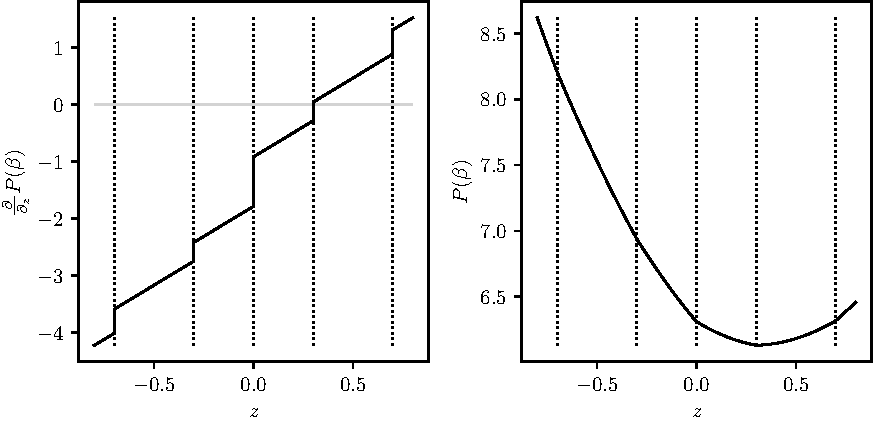
\includegraphics[]{clusterupdate-grad-obj}
  \caption{%
    Objective and gradient under the constraint that we have a fixed
    cluster.
    The optimum is found at \(\tilde\beta = 0.3\).
  }%
  \label{fig:cluster-grad-obj}
\end{figure}

Let \(\mathcal{B}\) be a cluster initialized to \(\mathcal{C}_k\), with
corresponding coefficient \(c_k\).
Then the coordinate update for \(\beta_\mathcal{B}\) is\jl{This obviously
does not work when \(s=0\). Can we just set \(s = 1\) here? It's just
the relative signs that really matter, right?}\jw{That is a really good point. Do you think we can tie to the sign of the gradient instead?. We also will not move the zero cluster this way suspect. But it should work for any formation then sign of the gradient is the way I think?}
\jl{Yes, I think you're right, in fact that's what I have in the code now.}
\[
  \beta_\mathcal{B} \gets
  s_\mathcal{B} \odot
    T \left(
      \frac{
        (y - \tilde y)^T X_{\mathcal{B}} s_{\mathcal{B}},
      }{
        s_{\mathcal{B}}^T X_{\mathcal{B}}^T X_{\mathcal{B}} s_{\mathcal{B}}
      } , 
      \frac{
        \lambda 
      }{
        s_{\mathcal{B}}^T X_{\mathcal{B}}^T X_{\mathcal{B}} s_{\mathcal{B}}
      } 
    \right)
\]
where
\begin{equation}
  \label{eq:slope-thresholding}
  T(a, \lambda) =
  \begin{cases}
    0                                                        & \text{if } |a| \leq \sum_{i=1}^{|\mathcal{B}|}\lambda^{C(0)}_i                                                                                                                      \\
    \sign(a)c_i                                              & \text{if } \sum_{j= |\mathcal{C}_i| - |\mathcal{B}|}^{|\mathcal{C}_i|} \lambda^{\mathcal{C}_i}_j \leq |a| - c_i \leq \sum_{j=1}^{|\mathcal{B}|}\lambda^{\mathcal{C}_i}_j \\
    \sign(a)\big(|a| - \sum_{j \in C(a)}\lambda_{(j)^-}\big) & \text{otherwise.
    }
  \end{cases}
\end{equation}
\JL{The third case cannot use \(C(a)\). We must think of something different.}
To emphasize the connection between \(T\) and the soft-thresholding operator
for the lasso, we call this operator the SLOPE-thresholding operator.
In \cref{fig:slope-thresholding}, we visualize the operator.

\begin{figure}[htbp]
  \centering
  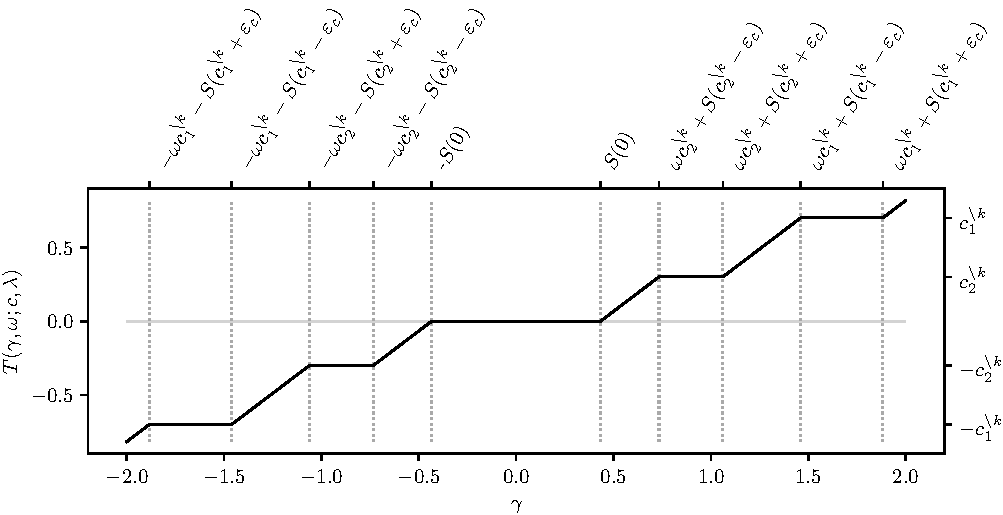
\includegraphics[]{slope-thresholding.pdf}
  \caption{The result of the SLOPE thresholding update.}
  \label{fig:slope-thresholding}
\end{figure}

\subsection{Algorithm}

Here is a rough sketch of a possible algorithm.
\begin{enumerate}
  \item Initialize \(\beta\) to zero.
  \item For each cluster,
        \begin{itemize}
          \item Check if the predictor with the largest correlation leaves the
                cluster, if not check if the two largest leave the cluster etc.
          \item If any predictors leave the cluster, compute the coordinate
                update for these predictors.
          \item If the cluster stays intact and does not correspond to the
                zero cluster, update the coefficient (common coordinate) for that
                cluster.
        \end{itemize}
\end{enumerate}
It is hopefully sufficient to only check if the coefficient with the
largest gradient splits from the cluster for most of the iterations since
checking all possible combinations of a cluster likely is expensive.
We have
to hope that's it's rare for multiple coefficients to leave a cluster in
a new cluster.

\section{EXPERIMENTS}\label{sec:experiments}
%%%%%%%%%%%%%%%%%%%%%%%%%%%%%%%%%%%%%%%%%%%

To investigate the performance of our algorithm, we performed an extensive benchmark against the following competitors:
\begin{itemize}[noitemsep]
  \item Alternating Direction Method of Multipliers (\texttt{ADMM})~\parencite{boyd2010}.
  We considered several alternative for the choice of the augmented Lagragian parameter: an adaptive method to update the parameter throughout the algorithm~\parencite[Sec. 3.4.1]{boyd2010} and fixed values.
  In the following sections, we only kept the \texttt{ADMM} solver with a fixed value of $100$ for the augmented Lagrangian parameter.
  We present in \Cref{sec:admm-benchmarks} a more detailed benchmarks for \texttt{ADMM} solvers with different values of this parameter and the adaptive setting.
  Choosing this parameter is not straightforward and the best value changes across datasets and regularization strengh.
  \item Anderson acceleration for proximal gradient descent (\texttt{anderson PGD})~\parencite{zhang2020}
  \item Proximal Gradient Descent (\texttt{PGD})~\parencite{combettes2005}
  \item Fast Iterative Shrinkage-Thresholding Algorithm (\texttt{FISTA})~\parencite{beck2009}
  \item Semismooth Newton-Based Augmented Lagrangian (\texttt{Newt-ALM})~\parencite{Ziyan2019}

  \item The hybrid (our) solver (see \Cref{alg:hybrid}) combines proximal gradient descent
        and coordinate descent to overcome the non-separability of the SLOPE problem.
  \item The Oracle solver (\texttt{oracle CD}) uses the clusters obtained via another solver to compute coordinate descent updates from the known solver.
  Note that it cannot be used in practice as it requires identifying the clusters of the minimizer of the SLOPE optimization problem \Cref{pb:slope}. This solver solves \Cref{pb:separable_slope} where clusters are obtained with the \texttt{hybrid} solver.
\end{itemize}

We used \pkg{Benchopt}~\parencite{moreau2022benchopt} to obtain the convergence curves for the different solvers.
\pkg{Benchopt} is a collaborative framework that allows reproducible and automatic benchmarks.
% This would void anonymity. We should uncomment for the camera-ready version.
% The repository to reproduce the benchmark is available at \url{https://github.com/Klopfe/benchmark_slope}.
The repository to reproduce the benchmark is available in the supplementary material.

Unless we note otherwise, we used the Benjamini--Hochberg method to compute the \(\lambda\) sequence~\parencite{bogdan2015},
which sets $\lambda_j = \eta^{-1}(1 - q\times j / (2p))$ for $j=1, 2, \hdots, p$ where $\eta^{-1}$ is the probit function.
For the rest of the experiments section, the parameter $q$ of this sequence has been set to $0.1$ if not stated otherwise.\footnote{We initially experimented with various settings for \(q\) but found that they made little difference to the relative performance of the algorithms.}
We let \(\lambda_\text{max}\) be the \(\lambda\) sequence such that \(\beta^* = 0\), but for which any scaling with a strictly positive scalar smaller than one produces a solution with at least one non-zero coefficient.
We then parameterize the experiments by scaling \(\lambda_\text{max}\), using the fixed factors \(1/2\), \(1/10\), and \(1/50\), which together cover the range of very sparse solutions to the almost-saturated case.

We pre-process datasets by first removing features with less than three non-zero values. Then, for dense data we center and scale each feature by its mean and standard deviation respectively.
For sparse data, we scale each feature by its maximum absolute value.

Each solver was coded in \pkg{python}, using \pkg{numpy}~\parencite{harris2020} and \pkg{numba}~\parencite{lam2015} for performance-critical code.
The code will be made open-source upon publication and is available in the supplementary material.

In \Cref{sec:solver-details}, we provide additional details on the implementations of some of the solvers used in our benchmarks.

The computations were carried out on a computing cluster with dual Intel Xeon CPUs (28 cores) and 128 GB of RAM.

\subsection{Simulated Data}
\label{sec:experiments-real-data}

\begin{figure*}[!t]
  \centering
  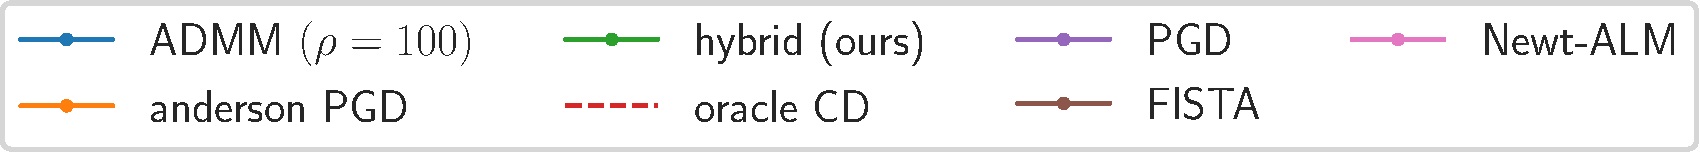
\includegraphics{simulated_legend.pdf}
  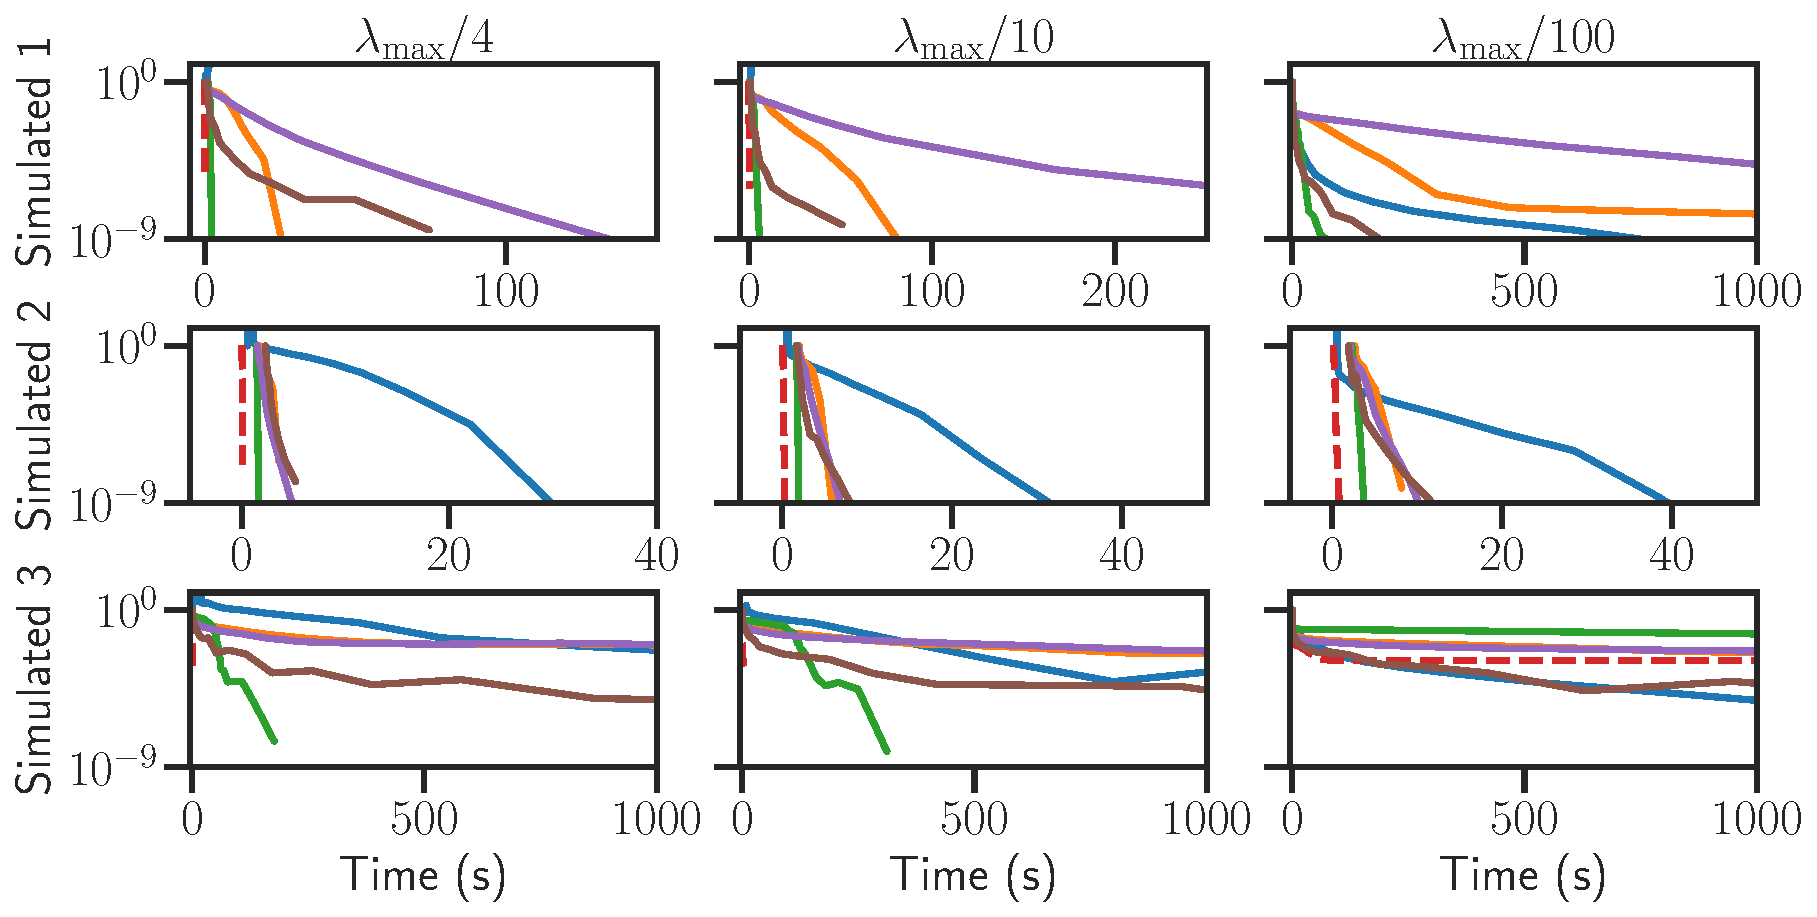
\includegraphics[scale=0.9]{simulated.pdf}
  \caption{Benchmark on simulated datasets. The plots show suboptimality as a function of time for SLOPE on multiple simulated datasets and $\lambda$ sequences of varying strength.}
  \label{fig:simulated}
\end{figure*}

The design matrix $X$ was generated such that features had mean one and unit variance, with correlation between features $j$ and $j'$ equal to $0.6^{|j-j'|}$.
%where $\rho$ is a parameter that can be chosen in $[0, 1[$.
%We fixed this value at $0.6$.
We generated \(\beta \in \mathbb{R}^p\) such that \(k\) entries, chosen uniformly at random throughout the vector, were sampled from a standard Gaussian distribution.
The response vector, meanwhile, was set to $y=X\beta + \varepsilon$, where
$\varepsilon$ was sampled from a multivariate Gaussian distribution with variance such that $\lVert X\beta\rVert / \lVert \varepsilon \rVert = 3$.

The different scenarios for the simulated data are described in \Cref{tab:simulated-data}

\begin{table}[hbt]
  \centering
  \caption{Scenarios for the simulated data in our benchmarks}
  \label{tab:simulated-data}
  \begin{tabular}{
      l
      S[table-format=5.0,round-mode=off]
      S[table-format=7.0,round-mode=off]
      S[table-format=2.0,round-mode=off]
      S[table-format=1.3,round-mode=off]
    }
    \toprule
    {Scenario} & {\(n\)} & {\(p\)} & {\(k\)} & {Density} \\ \midrule
    1          & 200     & 20000   & 20      & 1         \\
    2          & 20000   & 200     & 40      & 1         \\
    3          & 200     & 200000 & 20      & 0.001     \\ \bottomrule
  \end{tabular}
\end{table}

In \Cref{fig:simulated}, we present the results of the benchmarks on simulated data.
We see that for smaller fractions of $\lambda_{\text{max}}$ our hybrid algorithm allows significant speedup in comparison to its competitors mainly when the number of features is larger than the number of samples.
On very large scale data such as in simulated data setting $3$, we see that the hybrid solver is faster than its competitors by one or two orders of magnitude.


For the second scenario, notice that all solvers take considerably longer than the \texttt{oracle CD} method to reach convergence.
This gap is a consequence of Cholesky factorization in the case of \texttt{ADMM} and the global Lipschitz constant \(L\) in the remaining cases.
For the hybrid method, we can avoid this cost, with little impact on performance, since \(L\) is used only in the PGD step.
\mm{CHeck everywhere: we hare removed the notation $L$, it's the spectral norm of $X$ squared}

\subsection{Real data}
\label{sec:experiments-real-data}



The datasets used for the experiments have been described in \Cref{tab:real-data} and were obtained from \textcite{chang2011,chang2016,breheny2022}.

\begin{table}[hbt]
  \centering
  \caption{%
    List of real data sets used in our experiments.
    See \Cref{tab:dataset-sources} in \Cref{sec:dataset-sources} for references on these datasets.
  }
  \label{tab:real-data}
  \begin{tabular}{
      l
      S[table-format=5.0,round-mode=off]
      S[table-format=7.0,round-mode=off]
      S[table-format=1.5,round-mode=figures,round-precision=2]
    }
    \toprule
    Dataset            & {\(n\)} & {\(p\)} & {Density} \\ \midrule
    \dataset{bcTCGA}   & 536     & 17322   & 1         \\
    \dataset{news20}   & 19996   & 1355191 & 0.0003357 \\
    \dataset{rcv1}     & 20242   & 44504   & 0.00166   \\
    \dataset{Rhee2006} & 842     & 360     & 0.02469   \\ \bottomrule
  \end{tabular}
\end{table}

\Cref{fig:real-data} shows the suboptimality for the objective function $P$ as a function of the time for the four different datasets.
We see that when the regularization parameter is set at $\lambda_{\text{max}}/2$ and $\lambda_{\text{max}}/10$, our proposed solver is faster than all its competitors---especially when the datasets become larger.
This is especially visible for the \dataset{news20} dataset where we see that our proposed method is faster by at least one order of magnitude.

\begin{figure*}[!t]
  \centering
  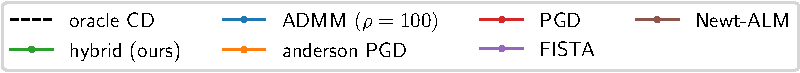
\includegraphics{real_legend.pdf}
  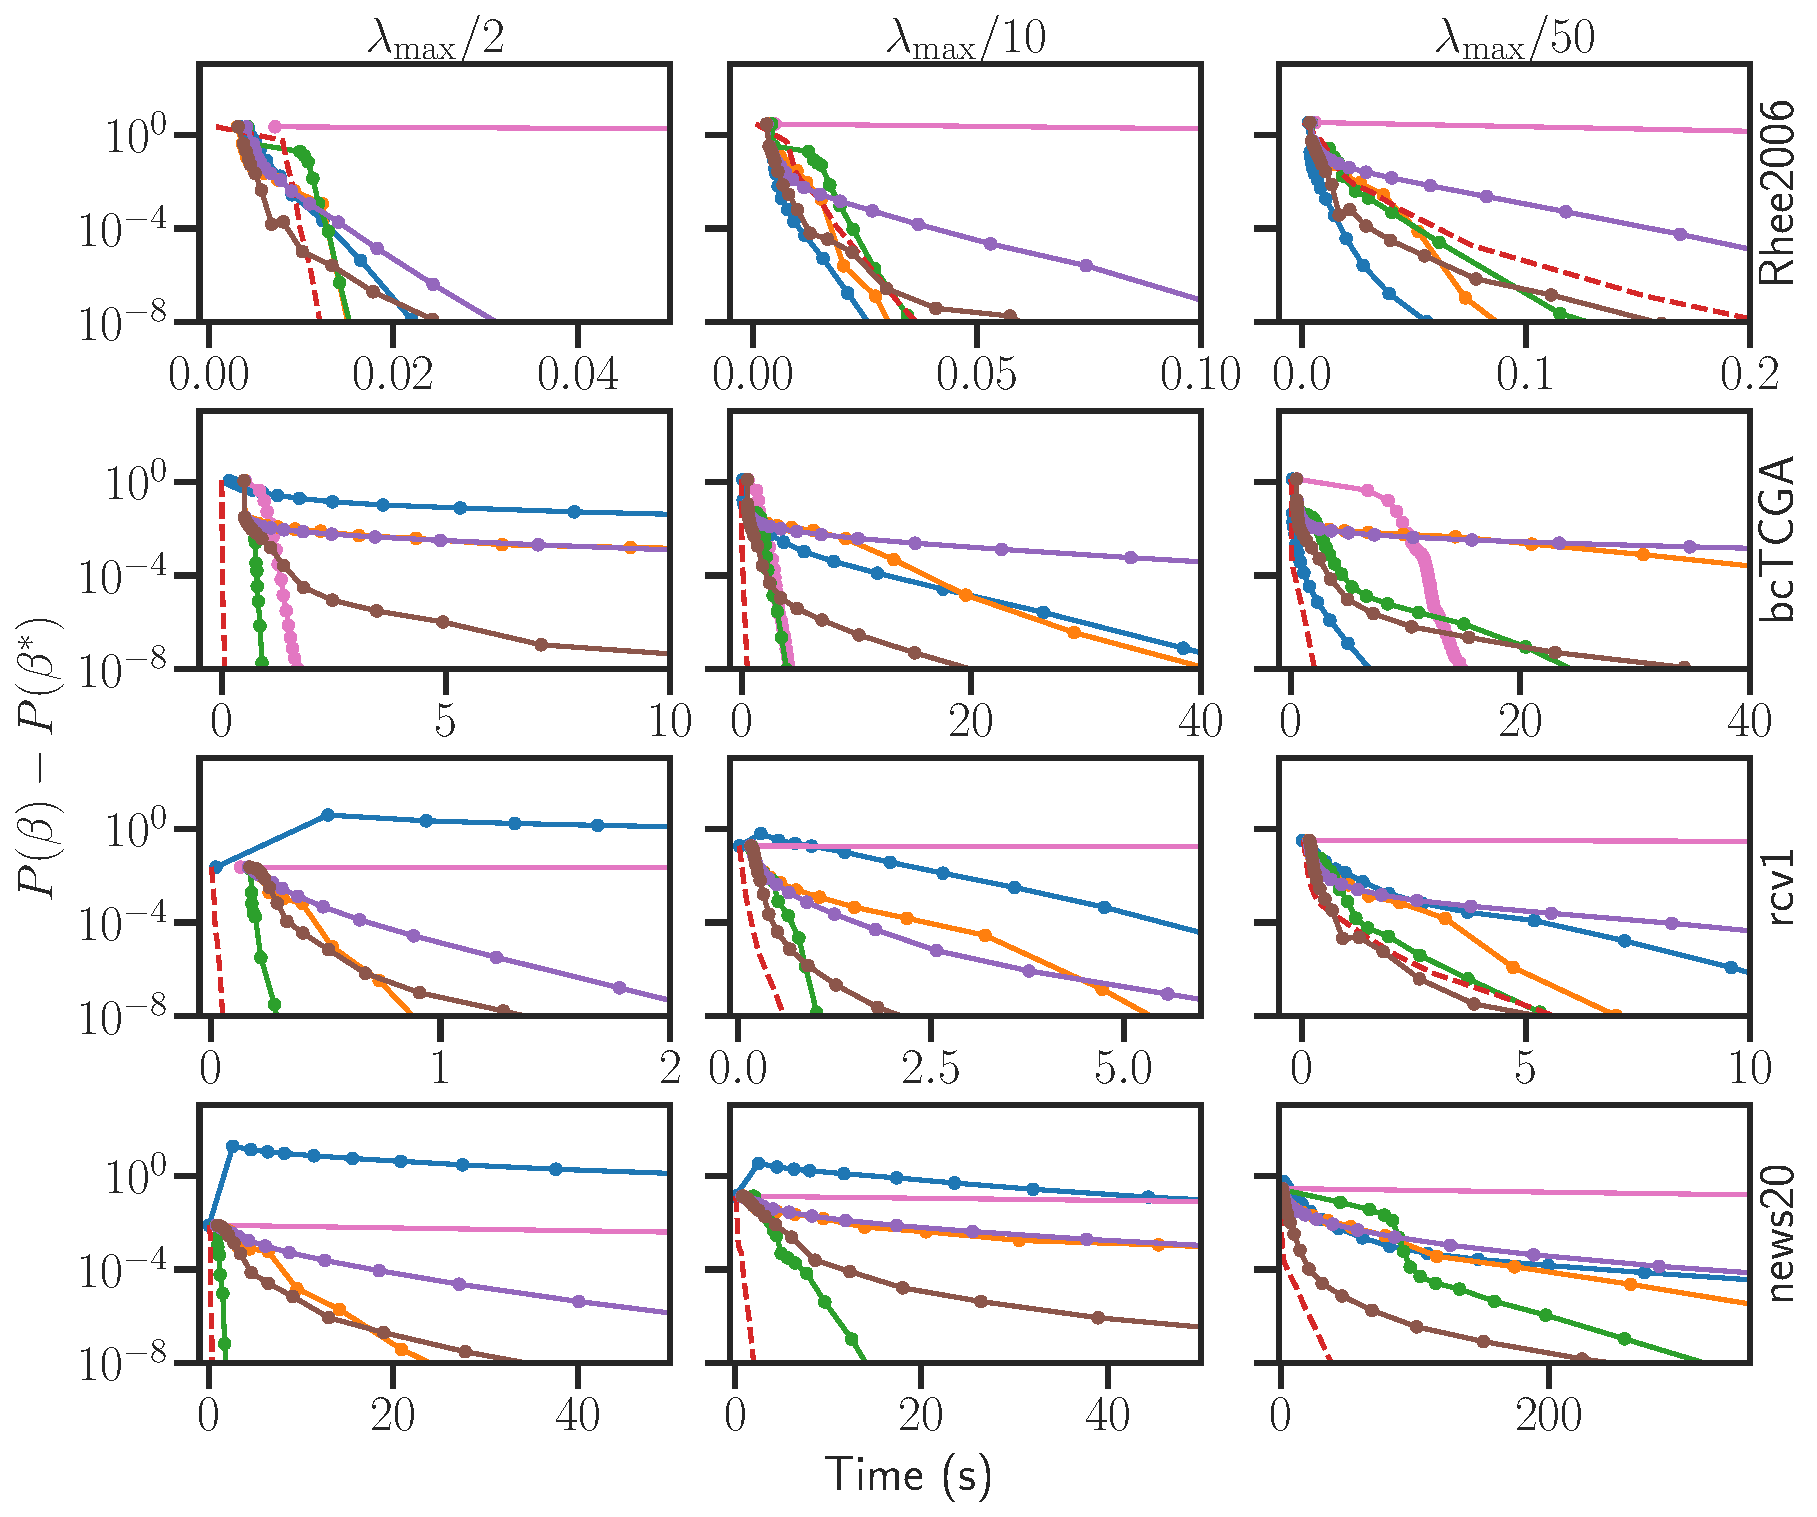
\includegraphics[scale=0.9]{real.pdf}
  \caption{Benchmark on real datasets. The plots show suboptimality as a function of time for SLOPE on multiple simulated datasets and $\lambda$ sequences of varying strength.}
  \label{fig:real-data}
\end{figure*}



When the parametrization value is set to $\lambda_{\text{max}}/50$, our algorithm remains competitive on the different datasets.
It can be seen that the different competitors do not behave consistently across the datasets.
For example, the \texttt{Newt-ALM} method is very fast on the \dataset{bcTCGA} dataset but is very slow on the \dataset{news20} dataset whereas the \texttt{hybrid} method remains very efficient in both settings.

As a final demonstration of the performance of our algorithm, we re-ran the experiment from the introduction on the \dataset{bcTCGA} dataset that took 43 seconds for the \pkg{SLOPE} package to reach convergence on.
Our algorithm, in contrast, reaches convergence in only 2.9 seconds\footnote{Note also that we do not use any screening rule in the current implementation of our algorithm, unlike the \pkg{SLOPE} package, which uses the strong screening rule for SLOPE~\parencite{larsson2020c}.}.
\mm{should this go to the introduction to tease the reader (rather than here where the reader is less focussed and we have already highlighted the superiority of the algo?)}

\section{DISCUSSION}\label{sec:discussion}
%%%%%%%%%%%%%%%%%%%%%%%%%%%%%%%%%%%%%%%%%

In this paper we have presented a new, fast algorithm for solving Sorted L-One Penalized Estimation (SLOPE).
Our method relies on a combination of proximal gradient descent to identify the cluster structure of the solution and coordinate descent to allow the algorithm to take large steps.
In our results, we have shown that our method often outperforms all competitors by orders of magnitude for high-to-medium levels of regularization and typically performs among the best algorithms for low levels of regularization.

We have not, in this paper, considered using screening rules for SLOPE~\parencite{larsson2020c,elvira2022}.
Although screening rules work for any algorithm considered in this article, they are particularly effective when used in tandem with coordinate descent~\parencite{fercoq2015} and, in addition, easy to implement due to the nature of coordinate descent steps.
Coordinate descent is moreover especially well-adapted to fitting a path of \(\lambda\) sequences~\parencite{friedman2007,friedman2010}, which is standard practice during cross-validating to obtain an optimal \(\lambda\) sequence.

Future research directions may include investigating alternative strategies to split clusters, for instance by considering the directional derivatives with respect to the coefficients of an entire cluster at once.
Another potential approach could be to see if the full proximal gradient steps might be replaced with batch stochastic gradient descent in order to reduce the costs of these steps.
Finally, it would also be interesting to consider whether gap safe screening rules might be used not only to screen predictors, but also to deduce whether clusters are able to change further during optimization.



\printbibliography

\appendix

\section{PROOFS}\label{sec:proofs}

\subsection{Proof of \Cref{thm:sl1-directional-derivative}}
\label{app:proof_directional_derivative}

Let \(c^{\setminus k}\) be the set containing all elements of $c$ except the $k$-th one: $c^{\setminus k} =  \{c_1, \ldots c_{k-1}, c_{k+1}, \ldots, c_m \}$.

From the observations in \Cref{rem:permutation_C_z},
we have the following cases to consider: \(|z| \in c^{\setminus k}\),
\(|z| = 0\), and \(|z| \notin \{0\} \cup c^{\setminus k}\).


\paragraph{Case 1}
Let us first consider the case $z \neq 0$, $|z| \neq c_i$ for all $i \neq k$.
Since \(C(z + \delta h) = C(z) = \cC_k\) and $\sign(z + \delta h) = \sign(z)$ for $h$ small enough,
\begin{align}
  H(z + \delta h) - H(z)
   & = \sum_{j =1}^p |\beta(z + \delta h)_j| \lambda_{(j)^-_{z + \delta h}}
  - \sum_{j=1}^p |\beta(z)_j| \lambda_{(j)^-_z} \nonumber                                       \\
   & = \sum_{j =1}^p (|\beta(z + \delta h)_j| - |\beta(z)_j|) \lambda_{(j)^-_z} \nonumber       \\
   & = \sum_{j =1}^p (|\beta(z + \delta h)_j| - |\beta(z)_j|) \lambda_{(j)^-_z} \nonumber       \\
   & = \sum_{j \in C(z)}^p (|\beta(z + \delta h)_j| - |\beta(z)_j|) \lambda_{(j)^-_z} \nonumber \\
   & = \sum_{j \in C(z)} \sign(\beta(z)_j) (z + \delta h - z) \lambda_{(j)^-_z} \nonumber       \\
   & = \sum_{j \in C(z)} \sign(z) \delta h  \lambda_{(j)^-_z} \nonumber                         \\
   & = \sum_{j \in \cC_k} \sign(z) \delta h  \lambda_{(j)^-_z} \, .
\end{align}

\paragraph{Case 2}
Then if  $z \neq 0$ and $|z|$ is equal to one of the $c_i$'s, $i \neq k$,  one has $C(z) = \cC_k \cup \cC_i$, $C(z + \delta h) = \cC_k$, and $\sign(z + \delta h) = \sign(z)$ for $h$ small enough.
Thus
\begin{align}
  H(z + \delta h) - H(z)
   & = \sum_{j =1}^p |\beta(z + \delta h)_j| \lambda_{(j)^-_{z + \delta h}}
  - \sum_{i=1}^p |\beta(z)_j| \lambda_{(j)^-_z}  \nonumber                                         \\
   & = \sum_{j \in \cC_k \cup \cC_i} \left( |\beta(z + \delta h)_j| \lambda_{(j)^-_{z + \delta h}}
  - |\beta(z)_j| \lambda_{(j)^-_z} \right)  \nonumber                                              \\
   & = \sum_{j \in \cC_k} \left( c_i + \delta h \right) \lambda_{(i)^-_{z + \delta h}}
  - c_i \lambda_{(i)^-_z}
  + \sum_{j \in \cC_i} \left( c_i \lambda_{(j)^-_{z + \delta h}}
    - c_i \lambda_{(i)^-_z} \right) \, .
\end{align}
\mm{to conclude we need to mention there is an ambiguity in terms of permutation (the permutation reordering $\beta(z)$ is not unique, we can swap $\cC_i$ and $\cC_k$, but it does not change the value of the sum, so we can pick $(i)_z = (i)_{z + \delta_h}$ and conclude) as above.}

\paragraph{Case 3} Finally let us treat the case $z = 0$.
If $c_m = 0$ then the proof proceeds as in case 2, with the exception that $|\beta(z + \delta h)| = h$ and so the result is just:
\begin{align}
  H(z + \delta h) - H(z)
   & = h \sum_{j \in \cC_k} \lambda_{(i)^-_{z + \delta h}} \, .
\end{align}
If $c_m \neq 0$, then the computation proceeds exactly as in case 1.

\subsection{Proof of \Cref{thm:thresholding-operator}}

Recall that \(G(z) : \mathbb{R} \to \mathbb{R}\) is a convex,
continuous piecewise-differentiable function with breakpoints whenever \(|z| =
c_i^{\setminus k}\) or \(z = 0\). Let \(\gamma = c_k \norm{\tilde{x}}^2+ \tilde x^Tr\)
and \(\omega = \norm{\tilde{x}}^2\) and note that the optimality criterion for
\eqref{pb:cluster-problem} is
\[
  \delta(\omega z - \gamma) + H'(z; \delta) \geq 0, \quad
  \forall \delta \in \{-1, 1\},
\]
which is equivalent to
\begin{equation}
  \label{eq:optimality-inequality}
  \omega z - H'(z; -1) \leq \gamma \leq \omega z + H'(z; 1).
\end{equation}
We now proceed to show that there is a solution \(z^* \in \argmin_{z \in
  \mathbb{R}} H(z)\) for every interval over \(\gamma \in \mathbb{R}\).

First, assume that the first case in the definition of \(T\) holds
and note that this is equivalent to \eqref{eq:optimality-inequality} with \(z
= 0\) since \(C({\varepsilon_c}) = C(-{\varepsilon_c})\) and
\(\lambda_{(j)^-_{-{\varepsilon_c}}} = \lambda_{(j)^-_{{\varepsilon_c}}}\).
This is sufficient for \(z^* = 0\).

Next, assume that the second case holds and observe that this is equivalent
to \eqref{eq:optimality-inequality} with
\(z = c_i^{\setminus k}\), since
\(C(c_i + {\varepsilon_c}) = C(-c_i - {\varepsilon_c})\) and
\(C(-c_i + {\varepsilon_c}) = C(c_i - {\varepsilon_c})\). Thus \(z^* =
\sign(\gamma)c_i^{\setminus k}\).

For the third case, we have
\[
  \smashoperator{\sum_{j \in C(c_i + {\varepsilon_c})}} \lambda_{(j)^-_{c_i + {\varepsilon_c}}}
  =
  \smashoperator[r]{\sum_{j \in C(c_{i-1} - {\varepsilon_c})}} \lambda_{(j)^-_{c_{i-1} - {\varepsilon_c}}}
\]
and therefore \eqref{eq:optimality-inequality} is equivalent to
\[
  c_i < \frac{1}{\omega} \bigg( |\gamma| - \smashoperator{\sum_{j \in C(c_i + {\varepsilon_c})}} \lambda_{(j)^-_{c_i + {\varepsilon_c}}} \bigg) < c_{i -1}.
\]
Now let
\begin{equation}
  \label{eq:differentiable-solution}
  z^* = \frac{\sign(\gamma)}{\omega} \bigg( |\gamma| - \smashoperator{\sum_{j \in C(c_i + {\varepsilon_c})}} \lambda_{(j)^-_{c_i + {\varepsilon_c}}} \bigg)
\end{equation}
and note that \(|z^*| \in \big(c_i^{\setminus k}, c_{i-1}^{\setminus k}\big)\) and hence
\[
  \frac{1}{\omega} \bigg( |\gamma| - \smashoperator{\sum_{j \in C(c_i + {\varepsilon_c})}} \lambda_{(j)^-_{c_i + {\varepsilon_c}}} \bigg)
  =
  \frac{1}{\omega} \bigg( |\gamma| - \smashoperator{\sum_{j \in C(z^*)}} \lambda_{(j)^-_{z^*}} \bigg).
\]
Furthermore, since \(G\) is differentiable in \(\big(c_i^{\setminus k}, c_{i-1}^{\setminus k}\big)\), we have
\[
  \frac{\partial}{\partial z} G(z) \Big|_{z = z^*}
  = \omega z^* - \gamma + \sign(z^*) \smashoperator{\sum_{j \in C(z^*)}} \lambda_{(j)^-_{z^*}} = 0,
\]
and therefore \eqref{eq:differentiable-solution} must be the solution.

The solution for the last case follows using reasoning analogous to that of the
third case.

\subsection{Proof of \Cref{lem:convergence}}

Let $\beta^*$ denote the stationary point of $F$.
If we denote the $t$th iteration of \Cref{alg:hybrid} as $T_t$, that is, $\beta^{(t+1)} = T_t(\beta^{t})$. Then by definition
$$
T_t(\beta)=\begin{cases}
T_{PGD}(\beta) & \mbox{if } t\bmod v=0, \\
T_{CD}(\beta) & \mbox{else,}  \\
\end{cases}
$$
where $T_{PGD}$ is an iteration proximal gradient descent and $T_{CD}$ is an iteration of coordinate descent. Clearly $P(T_{CD}(\beta)) \leq P(\beta)$. Now note that
$$
T_{PGD}(\beta)= \argmin_{\hat{\beta}} \left( H(\beta,\hat{\beta}) = f(\beta) + \langle \nabla f(\beta),\hat{\beta} - \beta ) + \frac{L(f)}{2} ||\beta-\hat{\beta}  ||^2+ J(\beta) \right)
$$ 
where $f(\beta) = \frac{1}{2} \norm{y - X \beta}^2$ and $L(f)$ is the Lipschitz constant. Note that by strong convexity that $H(\beta,T_{PGD}(\beta)) \leq F(T_{PGD}(\beta))$.
Then we can apply Lemma 3 in \textcite{richtarik2014}
to get
$$
P(T_{PGD}(\beta)) - P(\beta^*)  \leq 
\begin{cases}
\left(1 - \frac{P(\beta) - P(\beta^*)}{R^2} \right) \left( P(\beta) - P(\beta^*)\right) & \mbox{if } \left( P(\beta) - P(\beta^*) \right)\leq R^2, \\
\frac{1}{2}\left( P(\beta) - P(\beta^*)\right) & \mbox{else,}
\end{cases}
$$
where $R^2=||\beta- \beta^*||_L$. To get the convergence rate apply proof of Theorem 1 in \textcite{richtarik2014}.

\subsection{Partial smoothness of the sorted $\ell_1$ norm}
\label{app:sec:partly_smooth}
In this section, we prove that the sorted $\ell_1$ norm $J$ is partly smooth~\parencite{lewis2002a}.
This allows to apply result about the structure identification of the proximal gradient algorithm.

\begin{definition}
  Let $J$ be a proper closed convex function ad $x$ a point of its domain such that $\partial J(x) \neq \emptyset$.
  $J$ is said to be partly smooth at $x$ relative to a set $\cM$ containing x if:
  \begin{enumerate}
    \item $\cM$ is a $C^2$-manifold around $x$ and $J$ restricted to $\cM$ is $C^2$ around $x$
    \item The tangent space of $\cM$ at $x$ is the orthogonal of the linear hull of $\partial J(x)$.
    \item $\partial J$ is continuous at $x$ relative to $\cM$
  \end{enumerate}
\end{definition}

\begin{proposition}
  The sorted $\ell_1$ norm is partly smooth at any point of $\bbR^d$.
\end{proposition}

\begin{proof}
  % First, $J$ is convex and has full domain, so its subdifferential is always non-empty.
  % Let $x \in \bbR^d$.

  First, we consider the case where $| x_j| >0$ for all $j\in\bbR^d$.
  Let $m$ be the number of clusters of $x$ and $\cC_1, \ldots, \cC_m$ be those clusters, and let $c_1 > \ldots > c_m > 0$ be the  value of  $\lvert x \rvert$ on the clusters.

  We define $\varepsilon_c$ as in \Cref{eq:epsilon-c} and 
  let $\cB = \{u \in \bbR^d: \lVert u - x \rVert_\infty < \varepsilon_c / 2\}$.
  
  We will show that $J$ is partly smooth at $x$ relative to the subspace
  \begin{equation}
    \cM = \{ u \in \bbR^d : (\exists c' \in \bbR^m, \forall i \neq j \in [m], c'_i \neq c'_j) \& (\forall k \in [m], \forall j \in \cC_k, u_j = \sign(x_j) c'_k) \} \cap \cB \, .
  \end{equation}
  Moreover, let $v_k \in \bbR^d$ for $k \in [m]$  be equal to $\sign x_{\cC_k}$ on $\cC_k$ and to 0 outside, such that $x = \sum_{k=1}^m c_k v_k$.
  The set $\cM$ can then be rewritten as $\cM = \Span(v_1, \ldots v_m) \cap \cB$.
  One inclusion is trivial.
  For the other, let $u \in \Span(v_1, \ldots v_m) \cap \cB$.
  Then there exists $c' \in \bbR^k$, $u = \sum_{k=1}^m c'_k v_k$.
  Suppose that there exist $k \neq k'$ such that $c'_k = c'_{k'}$.
  Then since $\lVert x - u \rVert_\infty = \max_k |c_k - c'_k|$ and $|c_k - c_{k'}| > \varepsilon_c$, one has:
  \begin{align*}
     \varepsilon_c < |c_k - c_{k'}|
     &= |c_k - c'_k + c'_{k'} - c_{k'}| \\
     &\leq |c_k - c'_k| + |c'_{k'} - c_{k'}| \\
     &\leq 2 \lVert x - u \rVert_\infty \\
     &\leq  \varepsilon_c \, .
  \end{align*}

  This shows that clusters of any $u \in \cM$ are equal to clusters of $x$.
  In addition, the tangent space of $\cM$ at $x$ is $\Span(v_1, \hdots, v_m)$. 
  
  
  % $\{ u \in \bbR^d : (\exists c' \in \bbR^m, \forall i \neq j \in [d], c'_i \neq c'_j) \& (\forall k \in [m], \forall j \in \cC_k, |u_j| = c'_k) \}$.

  
%   $k(j):[d] \rightarrow [m]$  such that $j \in \cC_{k(j}$.
%  \begin{equation}
%     \cM = \{ u \in \bbR^d : u_j = \sign(x_j) c'_{k(j)}\mbox{ where }  c' \in \bbR^m, \forall i \neq l , c'_i \neq c'_l \} \cap \cB \, .
%   \end{equation}

\begin{enumerate}
  \item The set $\cM$ is then the intersection of a linear subspace and an open ball hence it is a $\cC^2$ manifold. 
  Following the observation of the fact that the clusters of any $u\in\cM$ are the same than the clusters of $x$, we have that 
  \begin{align}{}
    J(u) = \sum_{k=1}^m \left( \sum_{j \in \cC_k} \lambda_j \right)c_k' \enspace ,
  \end{align}
  hence $J$ is linear on $\cM$ thus $\cC^2$. 
  \item The subdifferential of $J$ at $x$ is 
  \begin{align}
    \partial J(x) = 
  \end{align}
  \klopfe{Compute what is the linear hull of subdifferential restricted to one cluster}
  \item The subdifferential of $J$ is a constant set locally around $x$ along $\cM$ which shows that it is continuous at $x$ relative to $\cM$. 
\end{enumerate}

% We will now establish that $J$ is linear on $\mathcal{M}$.
%   let $v_k \in \bbR^d$ for $k \in [m]$  be equal to $\sign x_{\cC_k}$ on $\cC_k$ and to 0 outside, such that $x = \sum_{k=1}^m c_k v_k$.

%   Note that for $u =\sum_{k=1}^m c'_k v_k\in \Span(v_1, \ldots v_m) \cap \cB$ the function $J(u) = \sum_{k=1}^m \left( \sum_{j \in \cC_k} \lambda_j \right)c_k'$ which is clearly linear hence 1 and 3 holds.




  $J$ is linear hence smooth on $\cM$, its gradient is TODO $\sum_k (\sum_{j \in \cC_k} \lambda_j) v_k$. \mm{and this is orthogonal to $\cM$ because??? it cannot be, it's in $\cM$}

  If one cluster of $x$ vanishes ($c_m = 0)$, the same reasoning holds wih the manifold $cM \cap \{u \in \bbR^d: u_{\cC_m} = 0\}$ aka $c'_m = 0$).
\end{proof}


\end{document}
